\apendice{Documentación técnica de programación}

\section{Introducción}
En esta sección vamos a detallar como preparar el entorno de desarrollo del proyecto y la estructura que forma.

Hay que tener en cuenta que en parte, también es un manual de usuario, puesto que el proyecto se ha desarrollado pensando en ser ejecutado desde el editor de \textit{Unity} debido a las facilidades que permite a la hora de modificar la escena, los elementos o las pruebas con diferentes parámetros de una forma rápida y directa.

\section{Estructura de directorios}
El proyecto tiene la siguiente estructura de directorios:

\begin{itemize}
\item \textbf{Build}: es el directorio con los ejecutables.
\item \textbf{Codigo\textbackslash Algoritmos\_de\_busqueda\_3D}: es el directorio raíz del proyecto en \textit{Unity}.
\item \textbf{Codigo\textbackslash Algoritmos\_de\_busqueda\_3D\textbackslash Assets}: en este directorio se encuentran todos los elementos que usamos en el proyecto en \textit{Unity}.
	\begin{itemize}
	\item \textbf{Editor\textbackslash Tests}: contiene los test del proyecto.
	\item \textbf{Escenas}: contiene las escenas del proyecto.
	\item \textbf{Materiales}: contiene los materiales creados.
	\item \textbf{Modelos}: contiene los modelos 3D usados.
	\item \textbf{Scripts}: contiene los archivos de código fuente.
	\item \textbf{Texturas}: contiene los texturas usadas.
	\end{itemize}
\item \textbf{Exportar}: es el directorio con el paquete de \textit{Unity} con el proyecto completo para importarlo a otro proyecto.
\item \textbf{Memoria}: contiene los archivos en latex con la memoria y los anexos.
\item \textbf{Vídeos}: contiene vídeos con distintos ejemplos.
\end{itemize}

A parte de los mencionados, hay más directorios y ficheros creados por \textit{Unity} para su funcionamiento.

\section{Manual del programador}
\subsection{Instalación de \textit{Unity}}

\textit{Unity} \cite{unityweb} en su versión linux puede instalarse de dos maneras: con el archivo .deb y a través de un instalador en forma de script. Ambos archivos se suministran desde la web oficial y se pueden obtener desde el siguiente enlace:

\href{https://forum.unity3d.com/threads/unity-on-linux-release-notes-and-known-issues.350256/}{Web oficial con las versiones de Unity para linux}\footnote{Web oficial Unity: \url{https://forum.unity3d.com/threads/unity-on-linux-release-notes-and-known-issues.350256/}}

La versión utilizada ha sido la 5.3.6f1 que se puede encontrar en:

\href{https://forum.unity3d.com/threads/unity-on-linux-release-notes-and-known-issues.350256/#post-2717623}{Post de la web oficial para la versión 5.3.6f1}\footnote{Unity 5.3.6f1: \url{https://forum.unity3d.com/threads/unity-on-linux-release-notes-and-known-issues.350256/\#post-2717623}}

Y descargar de los siguientes enlaces:

\begin{itemize}
\item Archivo deb: \href{http://download.unity3d.com/download_unity/linux/unity-editor-5.3.6f1+20160720_amd64.deb}{Archivo deb para versión 5.3.6f1}\footnote{Unity 5.3.6f1 archivo deb: \url{http://download.unity3d.com/download_unity/linux/unity-editor-5.3.6f1+20160720_amd64.deb}}

\item Instalador: \href{http://download.unity3d.com/download_unity/linux/unity-editor-installer-5.3.6f1+20160720.sh}{Instalador para versión 5.3.6f1}\footnote{Unity 5.3.6f1 instalador: \url{http://download.unity3d.com/download_unity/linux/unity-editor-installer-5.3.6f1+20160720.sh}}

\item Ambos archivos: \href{http://files.unity3d.com/levi/unity-editor-5.3.6f1+20160720.torrent}{Archivo torrent con ambos archivos}\footnote{Unity 5.3.6f1 ambos archivos: \url{http://files.unity3d.com/levi/unity-editor-5.3.6f1+20160720.torrent}}
\end{itemize}

Para realizar la instalación hemos usado el archivo instalador con los siguientes pasos:
\begin{enumerate}
\item Darle permisos de ejecución con chmod +x al archivo instalador
\item Ejecutar el archivo como superusuario. Crea un directorio donde lo ejecutemos donde se encontraran todos los archivos de Unity.
\end{enumerate}

Para ejecutarlo, hay que ir al nuevo directorio que creó el instalador y ejecutar el ejecutable del editor de Unity que se encuentra dentro de \textit{Editor/}. 

Para poder usar Monodevelop con la versión de \textit{Unity}, hay que instalar además de la versión que viene con el instalador, el resto de archivos de Monodevelop. Con el comando sudo \textit{apt-get install mono-complete} se instalan desde los repositorios todos los archivos necesarios.

Para comprobar que \textit{Unity} abrirá el Monodevelop con su versión para \textit{Unity}, desde el menú \textit{Edit->Preferences}, en la sección \textit{External Tools}, comprobamos que el editor de  los \textit{scripts} seleccionado es \textit{internal}. Aunque se puede usar cualquier editor para realizar los \textit{scripts}, es recomendable usar Monodevelop de esta forma porque hay diferencias entre los lenguajes de programación estándar y las versiones de ellos que usa \textit{Unity}.

También hace falta instalar librerías adicionales de MonoDevelop para poder usar el debugger. Podemos hacerlo desde un terminal con los siguientes comandos:
\begin{itemize}
\item \textit{sudo apt-get install mono-reference-assemblies-2.0}
\item \textit{sudo apt-get install mono-reference-assemblies-3.5}
\item \textit{sudo apt-get install mono-reference-assemblies-4.0}
\end{itemize}

Para usar el \textit{debugger} de MonoDevelop, hay que iniciar el proceso desde el editor de MonoDevelop, usando el botón de ejecución y las opciones de \textit{Debugger} y \textit{Unity Editor} como se ve en la figura \ref{fig:debuggermono}.

\begin{figure}[htpb]
    \centering
    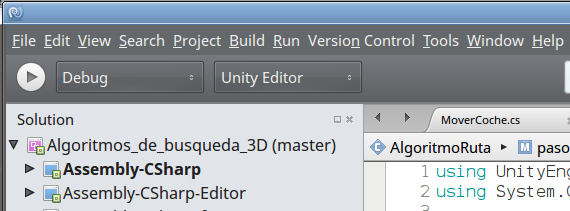
\includegraphics[width=\textwidth,height=4cm,keepaspectratio=true]{d_debuggermono}
    \caption[\textit{Debugger} para \textit{Unity Editor} de MonoDevelop]{\textit{Debugger} para \textit{Unity Editor} de MonoDevelop.}
    \label{fig:debuggermono}
\end{figure}

Entonces nos preguntará a que proceso de \textit{Unity Editor} queremos enlazarlo si no puede hacerlo el mismo. Seleccionamos el proceso de nuestro proyecto (podemos comprobar cual es con un gestor de procesos si no lo sabemos), y MonoDevelop quedará en espera. El proceso de \textit{debug} no comienza hasta que desde el \textit{Unity Editor} iniciemos la ejecución de forma normal, como lo haríamos sin el \textit{debugger}.

\begin{figure}[htpb]
    \centering
    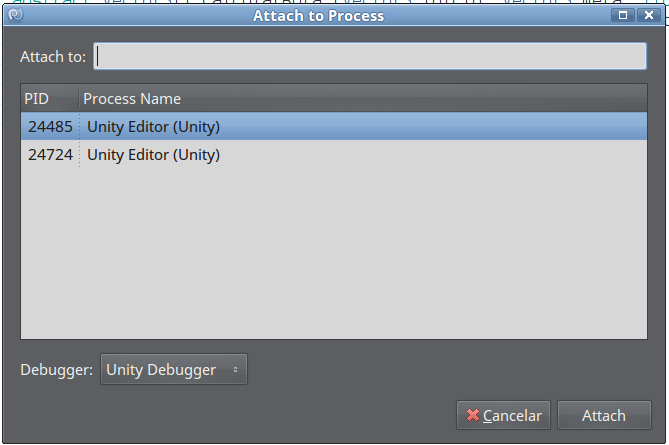
\includegraphics[width=\textwidth,height=6cm,keepaspectratio=true]{d_debuggermono2}
    \caption[Enlace del\textit{Debugger} con \textit{Unity Editor} de MonoDevelop]{Ventana donde se pregunta a que proceso de\textit{Unity Editor} enlazaremos el \textit{Debugger}.}
    \label{fig:debuggermono2}
\end{figure}

\subsection{Instalación SmartGit}

Para la organización del repositorio hemos elegido SmartGit, que es un programa disponible de forma gratuita para uso no comercial con versión para linux.

Para su instalación, hay que descargarse el archivo deb de su página web:

\href{https://www.syntevo.com/smartgit/download}{Página de SmartGit}\footnote{SmartGit: \url{https://www.syntevo.com/smartgit/download}}

La versión que hemos utilizado es la 17.0.3 que se puede descargar del siguiente enlace:

\href{https://www.syntevo.com/smartgit/download?file=smartgit/smartgit-17_0_3.deb}{Archivo deb de SmartGit 17.0.3}\footnote{SmartGit 17.0.3: \url{https://www.syntevo.com/smartgit/download?file=smartgit/smartgit-17_0_3.deb}}

El modo de instalación que hemos usado es haciendo doble \textit{click} sobre el archivo deb abriéndolo con el \textit{Instalador de software de Ubuntu}. También se puede instalar con el comando \textit{dpkg -i nombre-archivo.deb}.

\subsection{Instalación de Texmaker}
Texmaker lo hemos instalado desde los repositorios de Ubuntu usando el gestor con interfaz gráfica Synaptic.

También se puede instalar con el comando \textit{apt-get install textmaker}.

\subsection{Instalación ZenHub}

Para la planificación y control del proyecto hemos usado Zenhub sobre github. Es un complemento de Firefox que añade funciones como las \textit{boards} para manejar el control de las \textit{issues} y las \textit{milestones} del proyecto, y que permite ver los gráficos \textit{burndown} del progreso que se ha realizado.

Para instalarlo, hay que ir a la web oficial
\href{https://www.zenhub.com/}{Web oficial ZenHub}\footnote{Zenhub: \url{https://www.zenhub.com/}}

Pulsando sobre el botón de añadir ZenHub a Github, Firefox nos preguntará si queremos permitir a esa web instalar complementos, y debemos darle permiso. A continuación, se instalará en Firefox de forma automática y cuando vayamos a nuestro proyecto en github tendremos disponibles la funciones adicionales.

\subsection{Instalación de Remarkable}
Remarkable lo hemos usando el archivo deb descargado de la página oficial. La versión utilizada ha sido la 1.87, que se puede encontrar aquí:

\begin{itemize}
\item \href{https://remarkableapp.github.io/}{Página oficial}\footnote{Remarkable, página oficial: \url{https://remarkableapp.github.io/}}
\item \href{https://remarkableapp.github.io/files/remarkable_1.87_all.deb
}{Archivo deb}\footnote{Remarkable, archivo deb: \url{https://remarkableapp.github.io/files/remarkable_1.87_all.deb}}
\end{itemize}

También se puede instalar con el comando \textit{dpkg -i nombre-archivo.deb}.

\section{Compilación, instalación y ejecución del proyecto}
\subsection{Compilación}
El proceso de compilación de los \textit{scripts} se realiza automáticamente por el editor de \textit{Unity} cada vez que se realiza un cambio en alguno de ellos. Por tanto, no hay ningún comando o manera específica de hacerlo.

Para crear un archivo ejecutable con el proyecto, que irá acompañado de un directorio con los modelos y elementos necesarios para su ejecución, desde el editor de Unity vamos a \textit{File-\textgreater Build Settings}.

\begin{figure}[htpb]
    \centering
    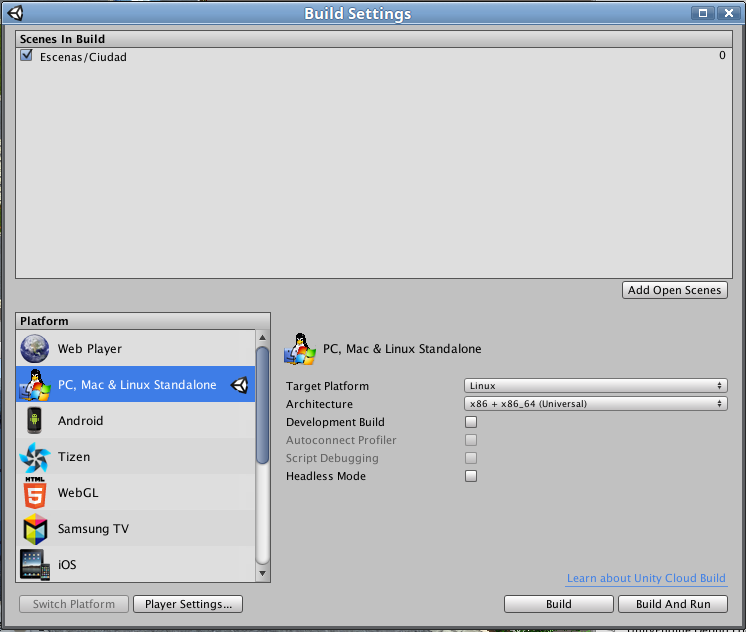
\includegraphics[width=\textwidth,height=8cm,keepaspectratio=true]{d_build}
    \caption[Menú de creación del ejecutable]{Ventana con las opciones de creación del ejecutable.}
    \label{fig:dbuild}
\end{figure}

Desde el menú de \textit{Build Settings}, elegimos las escenas que queramos incluir en el ejecutable, la plataforma en donde se ejecutará y el tipo de ejecutable que deseemos crear. A continuación, pulsamos en \textit{Build} y nos pedirá un nombre para el archivo y una ruta en donde se creará. Uan vez introducidos, comenzará el proceso de creación del archivo ejecutable.

\subsection{Instalación}\label{dinstalacion}
Para instalar el proyecto, el repositorio de Github con todos los ficheros necesarios es:
\href{https://github.com/vpe0001/Algoritmos\_de\_busqueda\_3D-Unity}{Repositorio del proyecto}\footnote{Repositorio del proyecto: \url{https://github.com/vpe0001/Algoritmos\_de\_busqueda\_3D-Unity}}

Con git o a través de la descarga del archivo zip, creamos una directorio con los archivos del proyecto. Desde \textit{Unity}, podemos abrir el proyecto que se encuentra en el directorio \textit{Codigo\textbackslash Algoritmos\_de\_busqueda\_3D}.

También se puede instalar desde \textit{Unity} después de crear un proyecto nuevo, desde el menú , importando el paquete de \textit{Unity} del directorio \textit{Exportar}.

\subsection{Ejecución}
Para ejecutarlo desde \textit{Unity}, hay que pulsar el botón de la flecha como podemos ver en la figura \ref{fig:dejecutar1}. Para parar la ejecución hay que volver a pulsar el botón de la flecha, y es posible pausarla con el boton de las dos barras verticales.

\begin{figure}[htpb]
    \centering
    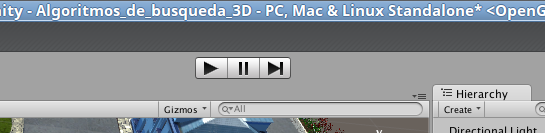
\includegraphics[width=\textwidth,height=8cm,keepaspectratio=true]{d_ejecutar}
    \caption[Botones de ejecución en \textit{Unity}]{Botones de ejecución en \textit{Unity}.}
    \label{fig:dejecutar1}
\end{figure}

\section{Pruebas del sistema}
Para la realización de los tests hemos usado la herramienta del editor de \textit{Unity}, que usa el \textit{framework} de NUnit. \textit{Unity} siempre va a buscar los archivos de tests en el directorio \textit{Editor}, y por ese motivo hemos colocado un directorio llamado \textit{Tests} dentro del mismo.

Para ejecutar los tests, desde el editor de \textit{Unity}, abrimos el \textit{Editor Test Runner} desde el menú \textit{Window}, y pulsamos sobre \textit{Run All} para realizarlos todos, o \textit{Run Selected} para ejecutar los tests concretos que se desee.

\begin{figure}[htpb]
    \centering
    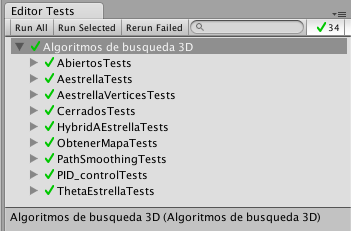
\includegraphics[width=\textwidth,height=6cm,keepaspectratio=true]{d_tests}
    \caption[Ejecución de tests en \textit{Unity}]{Ejecución de tests en \textit{Unity}.}
    \label{fig:dejecutar}
\end{figure}

Se han implementado casos de prueba para la mayoría de las clases, aunque por ejemplo, la clase MoverCoche no permite la realización de test debido a que al heredar de \textit{MonoBehaviour}, solo el Editor de \textit{Unity} puede instanciarla.

Para los tests de los algoritmos se ha realizado una búsqueda de ruta tanto si era posible alcanzar el destino, como si no lo era, dando lugar al error correspondiente.

Para las clases de los conjuntos de datos se ha comprobado que cada método realiza correctamente las operaciones de manipulación de los elementos que almacenan.

En el caso del \textit{Hybrid A*}, además de comprobar las rutas, se ha comprobado que los mapas que genera de obstáculos y de distancias son correctos.

En el PID\_Control se ha comprobado que los ángulos que calcula respecto a las posiciones del vehículo son correctos, y que los valores para un momento conocido para el movimiento del vehículo son los esperados.

En el \textit{PathSmoothing}, se ha comprobado que el descenso gradiente se obtienen los valores correctos al compararlos con los proporcionados por la documentación que se siguió para su implementación. Se comprobó que la eliminación del zigzag eliminaba estados que no eran necesarios, y que las curvas Bézier generan los puntos correctos y que sus valores eran los esperados.

En ObtenerMapa se comprobó que detectaba correctamente cuando una posición correspondía a un obstáculo y cuando no, y también se hicieron pruebas con los resultados obtenidos con la línea de visión para comprobar que el resultado era correcto.
